\documentclass{article}

\usepackage[margin=0.75in]{geometry}
\usepackage{graphicx}
\usepackage{amsmath}
\usepackage{float}
\usepackage[hidelinks]{hyperref}

\begin{document}

\title{Independent Smooth Signed Radial Kernel}
\author{}
\date{9 April 2026}
\maketitle
\footnotesize
\setlength{\parindent}{0pt}
\setlength{\parskip}{0.35em}

\section*{Approach}

The new method learns a radial kernel from scratch instead of initializing from a previously trained kernel. 
\noindent but the profile starts from a generic decaying curve. It is parameterized so that \(f_r\) stays nonnegative, nonincreasing, and unit-norm during training. The normalization used here is \(\lVert f \rVert_2 = 1\) during optimization. This prevents unstable growth and makes the profile easier to interpret.

The response is also changed from \texttt{abs\_max} to a signed top-\(k\) mean. The model computes the convolution map, keeps the strongest locations by absolute value, and averages their signed responses. I made this change to make the classification depend more on the learned kernel shape and less on a single magnitude peak.

The loss adds only the constraints needed to keep the profile well-behaved:
\begin{itemize}
    \item smoothness between neighboring shells,
    \item curvature regularization to suppress spikes,
    \item radial decay to reduce large outer-shell values,
    \item a final-shell penalty to push the tail toward zero.
\end{itemize}

Test accuracy = \(0.848\). \\
Test AUC = \(0.918725\).

\begin{figure}[H]
    \centering
    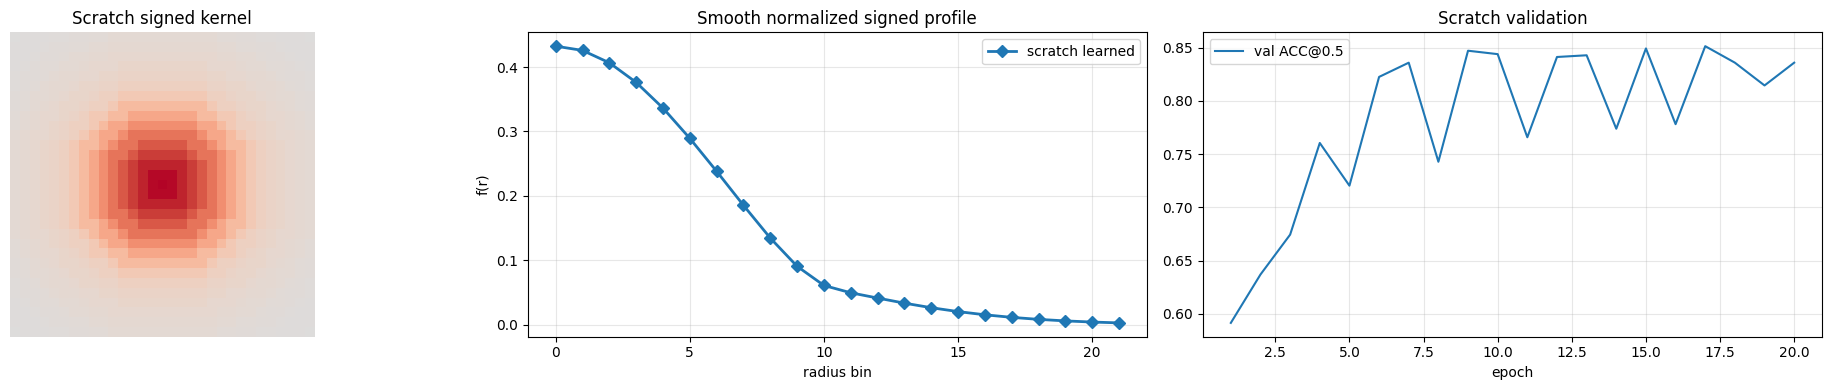
\includegraphics[width=\textwidth]{figures/radial_single_kernel_scratch_summary.png}
\end{figure}
\begin{figure}[H]
    \centering
    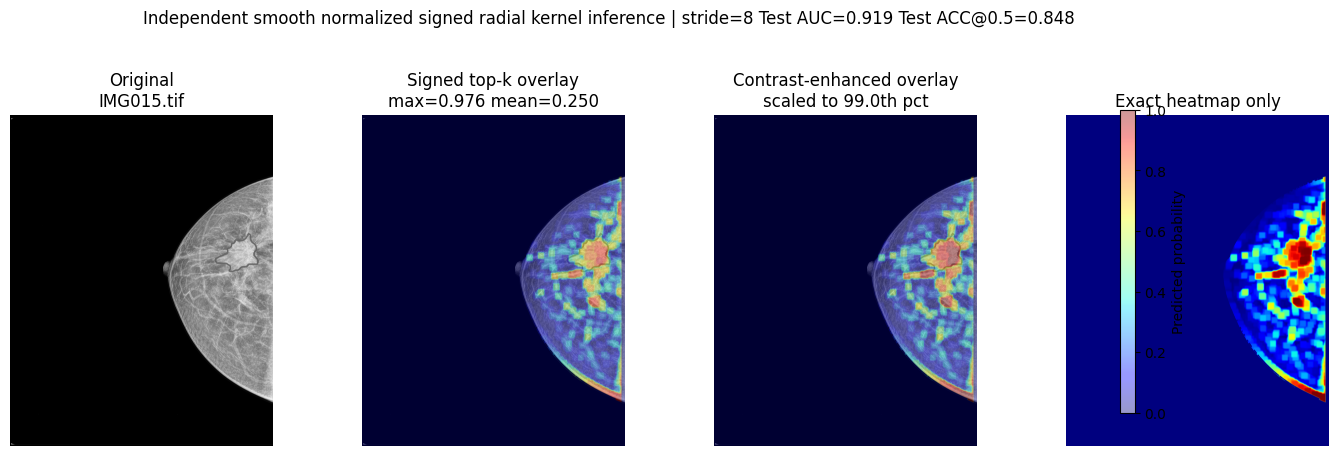
\includegraphics[width=\textwidth]{figures/radial_kernel_from_scratch_heatmap.png}
\end{figure}
\end{document}
